
%-----------------------------------------------------------------------------------------------------------------------------------------------%
%	The MIT License (MIT)
%
%	Copyright (c) 2019 Jan Küster
%
%	Permission is hereby granted, free of charge, to any person obtaining a copy
%	of this software and associated documentation files (the "Software"), to deal
%	in the Software without restriction, including without limitation the rights
%	to use, copy, modify, merge, publish, distribute, sublicense, and/or sell
%	copies of the Software, and to permit persons to whom the Software is
%	furnished to do so, subject to the following conditions:
%	
%	THE SOFTWARE IS PROVIDED "AS IS", WITHOUT WARRANTY OF ANY KIND, EXPRESS OR
%	IMPLIED, INCLUDING BUT NOT LIMITED TO THE WARRANTIES OF MERCHANTABILITY,
%	FITNESS FOR A PARTICULAR PURPOSE AND NONINFRINGEMENT. IN NO EVENT SHALL THE
%	AUTHORS OR COPYRIGHT HOLDERS BE LIABLE FOR ANY CLAIM, DAMAGES OR OTHER
%	LIABILITY, WHETHER IN AN ACTION OF CONTRACT, TORT OR OTHERWISE, ARISING FROM,
%	OUT OF OR IN CONNECTION WITH THE SOFTWARE OR THE USE OR OTHER DEALINGS IN
%	THE SOFTWARE.
%	
%
%-----------------------------------------------------------------------------------------------------------------------------------------------%


%============================================================================%
%
%	DOCUMENT DEFINITION
%
%============================================================================%

\documentclass[10pt,letterpaper,english]{article}	

%\documentclass[10pt,A4,english]{article}

%----------------------------------------------------------------------------------------
%	ENCODING
%----------------------------------------------------------------------------------------

% we use utf8 since we want to build from any machine
\usepackage[utf8]{inputenc}		
\usepackage[USenglish]{isodate}
\usepackage{fancyhdr}
\usepackage[numbers]{natbib}

%----------------------------------------------------------------------------------------
%	LOGIC
%----------------------------------------------------------------------------------------

% provides \isempty test
\usepackage{xstring, xifthen}
\usepackage{enumitem}
\usepackage[english]{babel}
\usepackage{blindtext}
\usepackage{pdfpages}
\usepackage{changepage}
%----------------------------------------------------------------------------------------
%	FONT BASICS
%----------------------------------------------------------------------------------------

% some tex-live fonts - choose your own

%\usepackage[defaultsans]{droidsans}
%\usepackage[default]{comfortaa}
%\usepackage{cmbright}
\usepackage[default]{raleway}
%\usepackage{fetamont}
%\usepackage[default]{gillius}
%\usepackage[light,math]{iwona}
%\usepackage[thin]{roboto} 

% set font default
\renewcommand*\familydefault{\sfdefault} 	
\usepackage[T1]{fontenc}

% more font size definitions
\usepackage{moresize}

%----------------------------------------------------------------------------------------
%	FONT AWESOME ICONS
%---------------------------------------------------------------------------------------- 

% include the fontawesome icon set
\usepackage{fontawesome}

% use to vertically center content
% credits to: http://tex.stackexchange.com/questions/7219/how-to-vertically-center-two-images-next-to-each-other
\newcommand{\vcenteredinclude}[1]{\begingroup
\setbox0=\hbox{\includegraphics{#1}}%
\parbox{\wd0}{\box0}\endgroup}
\newcommand{\tab}[1]{\hspace{.2\textwidth}\rlap{#1}}
% use to vertically center content
% credits to: http://tex.stackexchange.com/questions/7219/how-to-vertically-center-two-images-next-to-each-other
\newcommand*{\vcenteredhbox}[1]{\begingroup
\setbox0=\hbox{#1}\parbox{\wd0}{\box0}\endgroup}

% icon shortcut
\newcommand{\icon}[3] { 							
	\makebox(#2, #2){\textcolor{maincol}{\csname fa#1\endcsname}}
}	

% icon with text shortcut
\newcommand{\icontext}[4]{ 						
	\vcenteredhbox{\icon{#1}{#2}{#3}}  \hspace{2pt}  \parbox{0.9\mpwidth}{\textcolor{#4}{#3}}
}

% icon with website url
\newcommand{\iconhref}[5]{ 						
    \vcenteredhbox{\icon{#1}{#2}{#5}}  \hspace{2pt} \href{#4}{\textcolor{#5}{#3}}
}

% icon with email link
\newcommand{\iconemail}[5]{ 						
    \vcenteredhbox{\icon{#1}{#2}{#5}}  \hspace{2pt} \href{mailto:#4}{\textcolor{#5}{#3}}
}

%----------------------------------------------------------------------------------------
%	PAGE LAYOUT  DEFINITIONS
%----------------------------------------------------------------------------------------

% page outer frames (debug-only)
% \usepackage{showframe}		

% we use paracol to display breakable two columns
\usepackage{paracol}
\usepackage{tikzpagenodes}
\usetikzlibrary{calc}
\usepackage{lmodern}
\usepackage{multicol}
\usepackage{lipsum}
\usepackage{atbegshi}
% define page styles using geometry
\usepackage[letterpaper]{geometry} % letterpaper   % a4paper

% remove all possible margins
\geometry{top=1cm, bottom=1cm, left=1cm, right=1cm}

\usepackage{fancyhdr}
\pagestyle{empty}

% space between header and content
% \setlength{\headheight}{0pt}

% indentation is zero
\setlength{\parindent}{0mm}

%----------------------------------------------------------------------------------------
%	TABLE /ARRAY DEFINITIONS
%---------------------------------------------------------------------------------------- 

% extended aligning of tabular cells
\usepackage{array}

% custom column right-align with fixed width
% use like p{size} but via x{size}
\newcolumntype{x}[1]{%
>{\raggedleft\hspace{0pt}}p{#1}}%

%----------------------------------------------------------------------------------------
%	GRAPHICS DEFINITIONS
%---------------------------------------------------------------------------------------- 

%for header image
\usepackage{graphicx}

% use this for floating figures
% \usepackage{wrapfig}
% \usepackage{float}
% \floatstyle{boxed} 
% \restylefloat{figure}

%for drawing graphics		
\usepackage{tikz}			
\usepackage{ragged2e}	
\usetikzlibrary{shapes, backgrounds,mindmap, trees}

%----------------------------------------------------------------------------------------
%	Color DEFINITIONS
%---------------------------------------------------------------------------------------- 
\usepackage{transparent}
\usepackage{color}

% primary color
\definecolor{maincol}{RGB}{ 64,64,64}

% accent color, secondary
% \definecolor{accentcol}{RGB}{ 250, 150, 10 }

% dark color
\definecolor{darkcol}{RGB}{ 70, 70, 70 }

% light color
\definecolor{lightcol}{RGB}{245,245,245}

\definecolor{accentcol}{RGB}{20, 14, 57} % {59,77,97} % {20, 14, 57} {68,116,5}

% Package for links, must be the last package used
\usepackage[hidelinks]{hyperref}

% returns minipage width minus two times \fboxsep
% to keep padding included in width calculations
% can also be used for other boxes / environments
\newcommand{\mpwidth}{\linewidth-\fboxsep-\fboxsep}

%============================================================================%
%
%	CV COMMANDS
%
%============================================================================%

%----------------------------------------------------------------------------------------
%	 CV LIST
%----------------------------------------------------------------------------------------

% renders a standard latex list but abstracts away the environment definition (begin/end)
\newcommand{\cvlist}[1] {
	\begin{itemize}{#1}\end{itemize}
}

%----------------------------------------------------------------------------------------
%	 CV TEXT
%----------------------------------------------------------------------------------------

% base class to wrap any text based stuff here. Renders like a paragraph.
% Allows complex commands to be passed, too.
% param 1: *any
\newcommand{\cvtext}[1] {
	\begin{tabular*}{1\mpwidth}{p{0.98\mpwidth}}
		\parbox{1\mpwidth}{#1}
	\end{tabular*}
}
\newcommand{\cvtextsmall}[1] {
	\begin{tabular*}{0.8\mpwidth}{p{0.8\mpwidth}}
		\parbox{0.8\mpwidth}{#1}
	\end{tabular*}
}
%----------------------------------------------------------------------------------------
%	CV SECTION
%----------------------------------------------------------------------------------------

% Renders a a CV section headline with a nice underline in main color.
% param 1: section title
\newcommand{\cvsection}[1] {
	\vspace{14pt}
	\cvtext{
		\textbf{\LARGE{\textcolor{darkcol}{#1}}}\\[-4pt]
		\textcolor{accentcol}{ \rule{0.2\textwidth}{1.5pt} } \\
	}
}

\newcommand{\cvsectionsmall}[1] {
	\vspace{14pt}
	\cvtext{
		\textbf{\Large{\textcolor{darkcol}{#1}}}\\[-4pt]
		\textcolor{accentcol}{ \rule{0.2\textwidth}{1.5pt} } \\
	}
}

\newcommand{\cvheadline}[1] {
	\vspace{16pt}
	\cvtext{
		\textbf{\Huge{\textcolor{accentcol}{#1}}}\\[-4pt]
		 
	}
}

\newcommand{\cvsubheadline}[1] {
	\vspace{16pt}
	\cvtext{
		\textbf{\huge{\textcolor{darkcol}{#1}}}\\[-4pt]
		 
	}
}
%----------------------------------------------------------------------------------------
%	META SKILL
%----------------------------------------------------------------------------------------

% Renders a progress-bar to indicate a certain skill in percent.
% param 1: name of the skill / tech / etc.
% param 2: level (for example in years)
% param 3: percent, values range from 0 to 1
\newcommand{\cvskill}[3] {
	\begin{tabular*}{1\mpwidth}{p{0.72\mpwidth}  r}
 		\textcolor{black}{\textbf{#1}} & \textcolor{maincol}{#2}\\
	\end{tabular*}%
	
	\hspace{4pt}
	\begin{tikzpicture}[scale=1,rounded corners=2pt,very thin]
		\fill [lightcol] (0,0) rectangle (1\mpwidth, 0.15);
		\fill [accentcol] (0,0) rectangle (#3\mpwidth, 0.15);
  	\end{tikzpicture}%
}

%----------------------------------------------------------------------------------------
%	 CV EVENT
%----------------------------------------------------------------------------------------

% Renders a table and a paragraph (cvtext) wrapped in a parbox (to ensure minimum content
% is glued together when a pagebreak appears).
% Additional Information can be passed in text or list form (or other environments).
% the work you did
% param 1: time-frame i.e. Sep 14 - Jan 15 etc.
% param 2:	 event name (job position etc.)
% param 3: Customer, Employer, Industry
% param 4: Short description
% param 5: work done (optional)
% param 6: technologies include (optional)
% param 7: achievements (optional)
\newcommand{\cvevent}[7] {
	
	% we wrap this part in a parbox, so title and description are not separated on a pagebreak
	% if you need more control on page breaks, remove the parbox
	\parbox{\mpwidth}{
		\begin{tabular*}{1\mpwidth}{p{0.66\mpwidth}  r}
	 		\textcolor{black}{\textbf{#2}} & \colorbox{accentcol}{\makebox[0.32\mpwidth]{\textcolor{white}{\textbf{#1}}}} \\
			\textcolor{maincol}{#3} & \\
		\end{tabular*}\\[8pt]
	
		\ifthenelse{\isempty{#4}}{}{
			\cvtext{#4}\\
		}
	}
	\vspace{14pt}
}

%----------------------------------------------------------------------------------------
%	 CV META EVENT
%----------------------------------------------------------------------------------------

% Renders a CV event on the sidebar
% param 1: title
% param 2: subtitle (optional)
% param 3: customer, employer, etc,. (optional)
% param 4: info text (optional)
\newcommand{\cvmetaevent}[4] {
	\textcolor{maincol} { \cvtext{\textbf{\begin{flushleft}#1\end{flushleft}}}}

	\ifthenelse{\isempty{#2}}{}{
	\textcolor{black} {\cvtext{\textbf{#2}} }
	}

	\ifthenelse{\isempty{#3}}{}{
		\cvtext{{ \textcolor{maincol} {#3} }}\\
	}

	\cvtext{#4}\\[14pt]
}

%---------------------------------------------------------------------------------------
%	QR CODE
%----------------------------------------------------------------------------------------

% Renders a qrcode image (centered, relative to the parentwidth)
% param 1: percent width, from 0 to 1
\newcommand{\cvqrcode}[1] {
	\begin{center}
		\includegraphics[width={#1}\mpwidth]{qrcode}
	\end{center}
}

% HEADER AND FOOOTER 
%====================================
\newcommand\Header[1]{%
\begin{tikzpicture}[remember picture,overlay]
\fill[accentcol]
  (current page.north west) -- (current page.north east) --
  ([yshift=50pt]current page.north east|-current page text area.north east) --
  ([yshift=50pt,xshift=-3cm]current page.north|-current page text area.north) --
  ([yshift=10pt,xshift=-5cm]current page.north|-current page text area.north) --
  ([yshift=10pt]current page.north west|-current page text area.north west) -- cycle;
\node[font=\sffamily\bfseries\color{white},anchor=west,
  xshift=0.7cm,yshift=-0.32cm] at (current page.north west)
  {\fontsize{12}{12}\selectfont {#1}};
\end{tikzpicture}%
}

\newcommand\Footer[1]{%
\begin{tikzpicture}[remember picture,overlay]
\fill[lightcol]
  (current page.south east) -- (current page.south west) --
  ([yshift=-80pt]current page.south east|-current page text area.south east) --
  ([yshift=-80pt,xshift=-6cm]current page.south|-current page text area.south) --
  ([xshift=-2.5cm,yshift=-10pt]current page.south|-current page text area.south) --	
  ([yshift=-10pt]current page.south east|-current page text area.south east) -- cycle;
\node[yshift=0.32cm,xshift=9cm] at (current page.south) {\fontsize{10}{10}\selectfont \textbf{\thepage}};
\end{tikzpicture}%
}


%=====================================
%============================================================================%
%
%
%
%	DOCUMENT CONTENT
%
%
%
%============================================================================%
\begin{document}

\columnratio{0.31}
\setlength{\columnsep}{2.2em}
\setlength{\columnseprule}{4pt}
\colseprulecolor{white}


% LEBENSLAUF HIERE
\AtBeginShipoutFirst{\Header{CV}\Footer{1}} % CV
\AtBeginShipout{\AtBeginShipoutAddToBox{\Header{Curriculum Vitae}\Footer{2}}} % Curriculum Vitae

\newpage

\colseprulecolor{lightcol}
\columnratio{0.33} % 0.31
\setlength{\columnsep}{2.2em}
\setlength{\columnseprule}{4pt}
\begin{paracol}{2}


\begin{leftcolumn}
%---------------------------------------------------------------------------------------
%	META IMAGE
%----------------------------------------------------------------------------------------
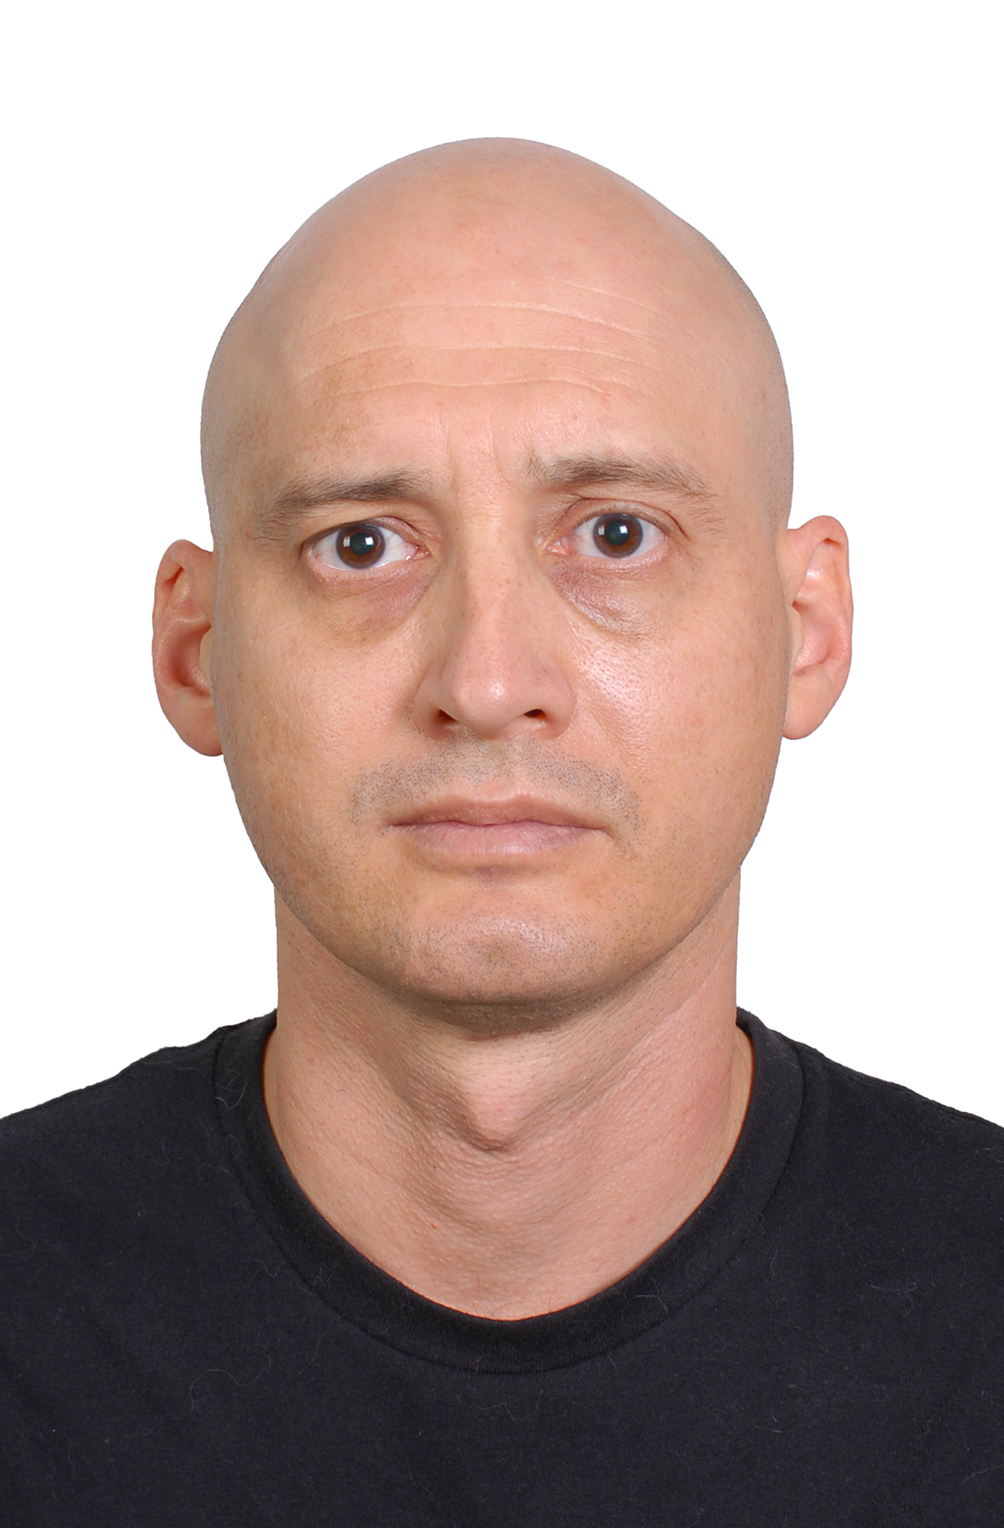
\includegraphics[width=\linewidth]{resources/MMENDEZ_Passportype.png}	%trimming relative to image size

%---------------------------------------------------------------------------------------
%	META SKILLS
%----------------------------------------------------------------------------------------
	\fcolorbox{white}{white}{\begin{minipage}[c][1.5cm][c]{1\mpwidth}
		\LARGE{\textbf{\textcolor{maincol}{Maikel Méndez-M}}} \\[2pt]
		\normalsize{ \textcolor{maincol} {Civil and Environmental Engineer (M.Sc.)} }
\end{minipage}} \\
\icontext{CaretRight}{12}{San José, Costa Rica}{black}\\[6pt]
\icontext{CaretRight}{12}{May/1975}{black}\\[6pt]
%\icontext{CaretRight}{12}{Single}{black}\\[6pt]

\cvsection{Skills}

\cvskill{Water Resources \newline Management} {20+ yrs.} {1.00} \\[-2pt]

\cvskill{Numerical Modelling} {20+ yrs.} {1.00} \\[-2pt]

%\cvskill{Remote Sensing (RS)/ \newline Geographic Information Systems (GIS)} {15+ yrs.} {0.75} \\[-2pt]

\cvskill{Remote Sensing + GIS} {15+ yrs.} {0.75} \\[-2pt]

\cvskill{Data Science} {10+ yrs.} {0.40} \\[-2pt]

\cvskill{Computational \newline Fluid Dynamics} {8+ yrs.} {0.36} \\[-2pt]

\cvskill{Climate Change} {8+ yrs.} {0.36} \\[-2pt]

\cvskill{Wastewater Treatment} {6+ yrs.} {0.30} \\[-2pt]

\cvskill{Irrigation + Drainage} {3+ yrs.} {0.20} \\[-2pt] \\

\cvskill{Language: Spanish} {L1} {1} \\[-2pt]

\cvskill{Language: English} {C2} {0.9} \\[-2pt]

%\newpage
%---------------------------------------------------------------------------------------
%	EDUCATION
%----------------------------------------------------------------------------------------
\cvsection{Education}

\cvmetaevent
{06/2009 - 07/2010}
{Geo-Information Science and Earth Observation (Postgraduate Degree)}
{Faculty of Geo-Information Science and Earth Observation (ITC). 
University of Twente, Enschede, The Netherlands}
{\textit{Geostatistics • R + Python Programming} \newline Thesis: \glqq "Parameterization and sensitivity analysis of the EPA-SWMM model for an urban catchment using Remote Sensing and PEST\grqq.}

\cvmetaevent
{09/2001 - 06/2003}
{Civil and Environmental Engineering (M.Sc.)}
{Arizona State University (ASU), Tempe, United States of America}
{\textit{Numerical Modelling • Hydrogeology} \newline Thesis: \glqq "An evaluation of the membrane fouling index (MFI) and its relevance to predict clogging in porous media\grqq.}

\cvmetaevent
{02/1993 - 02/1998}
{Agricultural Engineering (B.Sc.)}
{Instituto Tecnológico de Costa Rica, Campus Cartago, Costa Rica}
{\textit{Irrigation • Drainage} \newline Thesis: \glqq "Reservoir waterproofing of the Río-Lajas hydropower plant\grqq.}


%
%\cvsection{Projekte}

%	\cvlist{
%		\item \hyperlink{https://github.com/philipempl/ether-twin}{\textbf{Ether-Twin.}}\\ Ethereum Applikation für Digital Twins.
%		\item \hyperlink{https://github.com/philipempl/Peter-Pan}{\textbf{Peter Pan.}}\\ Koch-App (t.b.a.).
%		\item \hyperlink{https://github.com/philipempl/Innovation-Tool}{\textbf{Innovation Tool.}}\\ Webcrawler für \hyperlink{https://ibi.de/}{Ibi}.
%		\item \hyperlink{https://github.com/philipempl/cozone}{\textbf{COZONE.}} \\ Soziales Netzwerk (t.b.a.).
%		\item \hyperlink{https://github.com/geritwagner/enlit}{\textbf{ENLIT.}}\\ Exploring new Literature (Bachelorarbeit).
%		\item \textbf{Crowdfunding.} \\Modul mit \hyperlink{https://senacor.com/}{Senacor} für \hyperlink{https://www.paydirekt.de/}{paydirekt}.
%		}

%\newpage
%---------------------------------------------------------------------------------------
%	IT SKILLS
%----------------------------------------------------------------------------------------

\cvsection{IT Skills}

\icontext{CaretRight}{12}{GIS and Remote Sensing: GRASS, IDRISI, ILWIS, SAGA, QGIS}{black}\\[6pt]
\icontext{CaretRight}{12}{Water Resources: ModFLOW, HBV, HEC-HMS/RAS, TOPMODEL, SWAT, SWMM}{black}\\[6pt]
\icontext{CaretRight}{12}{Statistics and GeoStatistics: R, Python, Matlab}{black}\\[6pt]
\icontext{CaretRight}{12}{Computational Fluid Dynamics: OpenFOAM, COMSOL}{black}\\[6pt]
\icontext{CaretRight}{12}{Climate Change: PRECIS, RCA, RegCM, WRF}{black}\\[6pt]

%\newpage
%---------------------------------------------------------------------------------------
%	CONTACT
%----------------------------------------------------------------------------------------

\cvsection{Contact}

\icontext{MapMarker}{16}{Housing and Construction Research Center (CIVCO).  \newline Instituto Tecnológico de Costa Rica\\PO Box 159-7050, Cartago.  \newline Costa Rica}{black}\\[6pt]
\iconhref{Home}{16}{www.tec.ac.cr}{http://XXX-XXX.XXX.XX}{black}\\[6pt]
\icontext{MobilePhone}{16}{+506-2550-2425}{black}\\[6pt]
\iconemail{Envelope}{16}{mamendez@itcr.ac.cr}{maikel.mendez@gmail.com}{black}\\[6pt]
\iconemail{Envelope}{16}{maikel.mendez@gmail.com}{maikel.mendez@gmail.com}{black}\\[6pt]
\iconhref{Github}{16}{github.com/maikelonu}{https://www.github.com/username}{black}\\[6pt]
\iconhref{Youtube}{16}{www.youtube.com/maikelmendez}{https://www.xing.com/profile/User_Name}{black}\\
\iconhref{Trello}{16}{orcid.org/0000-0003-1919-141X}{https://www.xing.com/profile/User_Name}{black}\\	
\iconhref{Google}{16}{scholar.google.com/maikelmendez}{https://www.xing.com/profile/User_Name}{black}\\
% \iconhref{Xing}{16}{xing.com/user\_name}{https://www.xing.com/profile/User_Name}{black}\\

%\cvqrcode{0.3}

\end{leftcolumn}
\begin{rightcolumn}
%---------------------------------------------------------------------------------------
%	TITLE  HEADER
%----------------------------------------------------------------------------------------


%---------------------------------------------------------------------------------------
%	PROFILE
%----------------------------------------------------------------------------------------
\cvsection{Biography}
\vspace{8pt} %4

\cvtext{Maikel Méndez is a Senior Lecturer and Researcher in Water Resources at the Construction Engineering School, Costa Rica Institute of Technology (TEC). Maikel's research focuses on Climate Change, Hydrological Modelling, Remote Sensing, GIS Integration, Machine Learning, Data Mining, and Computational Fluid Dynamics. Maikel is the leading author of various scientific publications that have contributed to finding solutions to complex problems and have also been incorporated into Costa Rican legislation. Maikel holds an M.Sc. in Civil and Environmental Engineering (ASU), a Postgraduate Degree in Earth Observation (U-TWENTE), and a major in Agricultural Engineering (TEC).}


%---------------------------------------------------------------------------------------
%	WORK EXPERIENCE
%---------------------------------------------------------------------------------------

\vspace{10pt}
\cvsection{Experience}
\vspace{4pt}

\cvevent
{06/2005 - Today}
	{Professor | Researcher}
	{Construction Engineering School\newline Instituto Tecnológico de Costa Rica (TEC) \newline https://www.tec.ac.cr}
	{Research in the areas of: Water Resources Management, Climate Change and Data Science. Lectures on: Hydraulics and Fluid Mechanics, Hydrology, Applied Statistics and Numerical Mathematics.}
	\vfill\null

\cvevent
{01/2000 - 05/2005}
	{Operations Engineer}
	{Operations Department\newline Instituto Costarricense de Acueductos y Alcantarillados \newline https://www.aya.go.cr}
	{Design, construction and operation of Water and Wastewater Facilities.}
	\vfill\null

\cvevent
{04/1998 - 11/1999}
	{Field Engineer}
	{Development Department\newline Linda Vista / Ball Horticultural Company \newline https:// www.ballhort.com}
	{Design, construction and operation of Irrigation and Drainage Systems.}
	\vfill\null

\cvevent
{11/1997 - 04/1998}
	{Irrigation Engineer}
	{Irrigation Department\newline Amanco-Plásticos para la Construcción \newline https://www.wavin.com}
	{Design, construction and operation of Irrigation Systems.}
	\vfill\null

\cvevent
{05/2003 - 12/2003}
	{Internship}
	{Department of Economic and Social Affairs (DESA) \newline United Nations Headquarters (NYC) \newline https://www.un.org/en/desa}
	{Research assistant in the fields of Hydrology, Applied Statistics and Environmental Accounting.}
	\vfill\null

\newpage

%---------------------------------------------------------------------------------------
%	PUBLICATIONS
%---------------------------------------------------------------------------------------

\vspace{10pt}
\cvsection{Publications}
\vspace{4pt}

\begin{itemize}[leftmargin=*]

\item Mendez, M.,Calvo-Valverde, L.A., Hidalgo-Madriz, J.A \& Araya-Obando, J.A. (2023). A comparison of generalized extreme value, gumbel, and log-pearson distributions for the development of intensity duration frequency curves. A case study in Costa Rica". In: \textit{edp-sciences BIO Web Conf}, 62(2023), 01002, 2022. \newline https://doi.org/10.1051/bioconf/20236201002.
\item Mendez, M., Maathuis, B.,Calvo-Valverde, L.A. \& Alvarado-Gamboa, L.F. (2022). "Hydrological Response of Tropical Catchments to Climate Change as Modeled by the GR2M Model: A Case Study in Costa Rica". In: \textit{Sustainability}, 14(24), 16938, 2022. \newline https://doi.org/10.3390/su142416938.
\item Mendez, M., Maathuis, B., Hein-Griggs, D. \& Alvarado-Gamboa, L.F. (2020). "Performance evaluation of bias correction methods for climate change monthly precipitation projections over Costa Rica". In: \textit{Water}, 12(2), 482, 2020. \newline https://doi.org/10.3390/w12020482.
\item Mendez, M. \& Calvo-Valverde, L.A. (2020). "Comparison performance of machine learning and geostatistical methods for the interpolation of monthly air temperature over Costa Rica". In: \textit{IOP Conference Series: Earth and Environmental Science (EES)}, 432, 2020. \newline https://doi.org/10.1088/1755-1315/432/1/012011.
\item Arriola-Valverde, S., Villagra-Mendoza, K., \& Mendez, M. (2020). "Analysis of Crop Dynamics through Close-Range UAS Photogrammetry". In: \textit{IEEE International Symposium on Circuits and Systems (ISCAS)}, 2020. \newline https://doi.org/10.1109/ISCAS45731.2020.9181285.
\item Mendez, M., Maathuis, B., Hein-Griggs, D. \& Alvarado-Gamboa, L.F. (2019). "Generation of Monthly Precipitation Climatologies for Costa Rica Using Irregular Rain-Gauge Observational Networks". In: \textit{Water}, 11(1), 70, 2019. \newline https://doi.org/10.3390/w11010070.
\item Hernandez-Castro, F., Monge-Fallas, J., Mendez, M. \& Segura-Solis, D. (2019). "Costa Rica: Visualization of the Movements of the Earth’s Crust". In: \textit{PONTE. International Journal of Sciences and Research}, 75, 2019. \newline https://doi.org/10.21506/j.ponte.2019.4.1.
\item Mendez, M. \& Calvo-Valverde, L.A. (2019). "Comparison of global and local optimization methods for the calibration and sensitivity analysis of a conceptual hydrological model". In: \textit{Tecnología en Marcha}, 32, 24-36, 2019. \newline https://doi.org/10.18845/tm.v32i3.4477.
\item Arriola-Valverde, S., Villagra-Mendoza, K., \& Mendez, M. (2019). "Desarrollo y Validación de una Metodología para la Cuantificación de la Erosión Hídrica a través de Fotogrametría UAS". In: \textit{Tecnología en Marcha}, 32, 43-52, 2019. \newline https://doi.org/10.18845/tm.v32i5.4171.
\item Hernandez-Castro, F., Monge-Fallas, J., Mendez, M. \& Protti-Quesada, M. (2018). "Animation: Crustal Deformation in the Nicoya Peninsula Associated with the September 5th, 2012 Earthquake". In: \textit{Scientific Visualization}, 10(3), 2018. \newline https://doi.org/10.26583/sv.10.3.09.
\item Mendez, M. \& Calvo-Valverde, L.A. (2016). "Development of the HBV-TEC Hydrological Model". In: \textit{Procedia Engineering}, 154, 1116-1123, 2016. \newline https://doi.org/10.1016/j.proeng.2016.07.521.
\item Mendez, M. \& Calvo-Valverde, L.A. (2016). "Assessing the performance of several rainfall interpolation methods as evaluated by a conceptual hydrological model". In: \textit{Procedia Engineering}, 154, 1050-1057, 2016. \newline https://doi.org/10.1016/j.proeng.2016.07.595.
\item Mendez, M. (2014). "Hydrologic and Hydraulic Assessment of Small Tropical Urban Catchments: A Case Study in Costa Rica". In: \textit{Proceedings of the 13th International Conference on Urban Drainage}, 15-16, 2014. \newline https://doi.org/10.1016/j.proeng.2016.07.595.
\item Mendez, M. (2014). "Diseño óptimo de un sistema de distribución de agua (SDA) aplicando el algoritmo Simulated Annealing (SA)". In: \textit{Tecnología en Marcha}, 23-31, 2014. \newline https://doi.org/10.18845/tm.v27i3.2063.
\item Mendez, M., Araya, J.A., \& Sánchez, L.D. (2013). "Automated parameter optimization of a water distribution system". In: \textit{Journal of Hydroinformatics}, 15 (1), 71-85, 2013. \newline https://doi.org/10.2166/hydro.2012.028.
\item Mendez, M. (2013). "Calibración y validación del modelo hidrológico SWMM en cuencas hidrográficas  de alta pendiente en Costa Rica". In: \textit{Tecnología en Marcha}, 20-32, 2013. \newline https://doi.org/10.18845/tm.v26i2.1400.
\item Mendez, M. (2013). "Predicción del impacto del cambio temporal del uso del suelo sobre cuencas hidrológicas de alta pendiente en Costa Rica". In: \textit{Tecnología en Marcha}, 13-25, 26, 2013. \newline https://doi.org/10.18845/tm.v26i3.1514.
\item Mendez, M. (2013). "Generación de Modelos de Elevación Digital (DEMs) a partir de análisis fotogramétrico haciendo uso de las imágenes CARTA-2005". In: \textit{Tecnología en Marcha}, 26-31, 26, 2013. \newline https://doi.org/10.18845/tm.v26i4.1578.
\item Mendez, M. (2008). "Modelación Asistida de Sistemas de Distribución de Agua (MASDA). Caso de estudio: Acueducto Marsella". In: \textit{Tecnología en Marcha}, 79-91, 21, 2008. %\newline https:// revistas.tec.ac.cr/index.php/tec_marcha/article/view/229/.
\item Mendez, M. (2007). "Modelación Asistida de Sistemas de Distribución de Agua (MASDA). Caso de estudio: campo/escuela Scout de Costa Rica". In: \textit{Tecnología en Marcha}, 12-23, 19, 2007. %\newline https://doi.org/10.18845/tm.v26i4.1578.
\end{itemize}

%---------------------------------------------------------------------------------------
%	CONFERENCES
%---------------------------------------------------------------------------------------

\vspace{10pt}
\cvsection{Conferences}
\vspace{4pt}

\begin{itemize}[leftmargin=*]

\item International Conference on Environment, Resources and Energy Engineering (EREE), Bangkok, Thailand
\textit{(2023)}.

\item International Conference on Resources and Environmental Research (ICRER), Shandong University, Qingdao, China \textit{(2019)}.

\item 37th IAHR Water World congress. Kuala Lumpur, Malaysia. \textit{(2017)}.

\item 12th International Conference on Hydroinformatics (HIC 2016). Incheon, Korea. \textit{(2015)}.

\item MetOffice: Regional Climate Change Model PRECIS, Exeter, United Kingdom. \textit{(2015)}

\item 13th International Conference on Urban Drainage 2014 (ICUD 2014). Sarawak, Borneo, Malaysia. \textit{(2014)}.

\item PREVDA: Programa Regional de Reducción de la Vulnerabilidad y Degradación Ambiental.Ciudad de Panamá, Panamá \textit{(2010)}.

\item AECID, Agencia Española de Cooperación Internacional y Desarrollo. Centro de Estudios Hidrográficos-CEDEX. Cartagena de Indias. Colombia \textit{(2008)}.

\end{itemize}


%---------------------------------------------------------------------------------------
%	FELLOWSHIPS 
%---------------------------------------------------------------------------------------

\vspace{10pt}
\cvsection{Fellowships}
\vspace{2pt}

\begin{itemize}[leftmargin=*]

\item NUFFIC, Netherlands Fellowship Programmes. \textit{(2009)}.

\item IIE-United Nations Fellowship Program, NYC. \textit{(2003)}.

\item Fulbright: Academic and Professional Programs for the Americas Fulbright Graduate Fellowship Program \textit{(2001)}.

\end{itemize}

%Modified, \today     \hspace{1cm}   \hrulefill

%\hspace*{30mm}\phantom{Lorem, \today }Maikel Mendez-M

\end{rightcolumn}
\end{paracol}


\end{document}